\documentclass{article}
\usepackage[utf8]{inputenc}
\usepackage[pdftex]{graphicx}
\usepackage{amsmath}
\usepackage{amsfonts}
\usepackage{amssymb}
\usepackage{pdfpages}
\usepackage[font=small]{caption}
\usepackage{float}
\usepackage{comment}
\usepackage{setspace}
\usepackage{textcomp}
\usepackage{gensymb}
\usepackage{multicol}
\usepackage{fancyhdr}
\usepackage{enumitem}
\usepackage{mathtools}
\usepackage{caption}
\usepackage{subcaption}
\usepackage{longtable}
\usepackage[margin=1in]{geometry}
\setlength{\parindent}{0pt}

\begin{document}

\begin{center}
\huge{Final Project Technical Report} \\
\small{Vishnu Gottiparthy (vtg4), Alexander Blumenstock (ab546)} \\
ECE 350L: Digital Systems\\
December 15, 2017 \\
\end{center}

\section{Motivation}
This project is a light-sensitive robotic arm with an infrared remote control and VGA display. The arm could automate keeping the lights on in a room, and could take custom actions set by the user when triggered by light level. The action being taken is indicated by a color change on the VGA display.

\section{Design}
    \subsection{Overview}
    This project consists of an FPGA running a ECE 350 processor, a robotic arm with voltage amplifier circuit, a light sensor circuit, and an infrared remote control. Figure \ref{fig:setup} shows the full setup for the project.
    
    \begin{figure}[H]
        \centering
        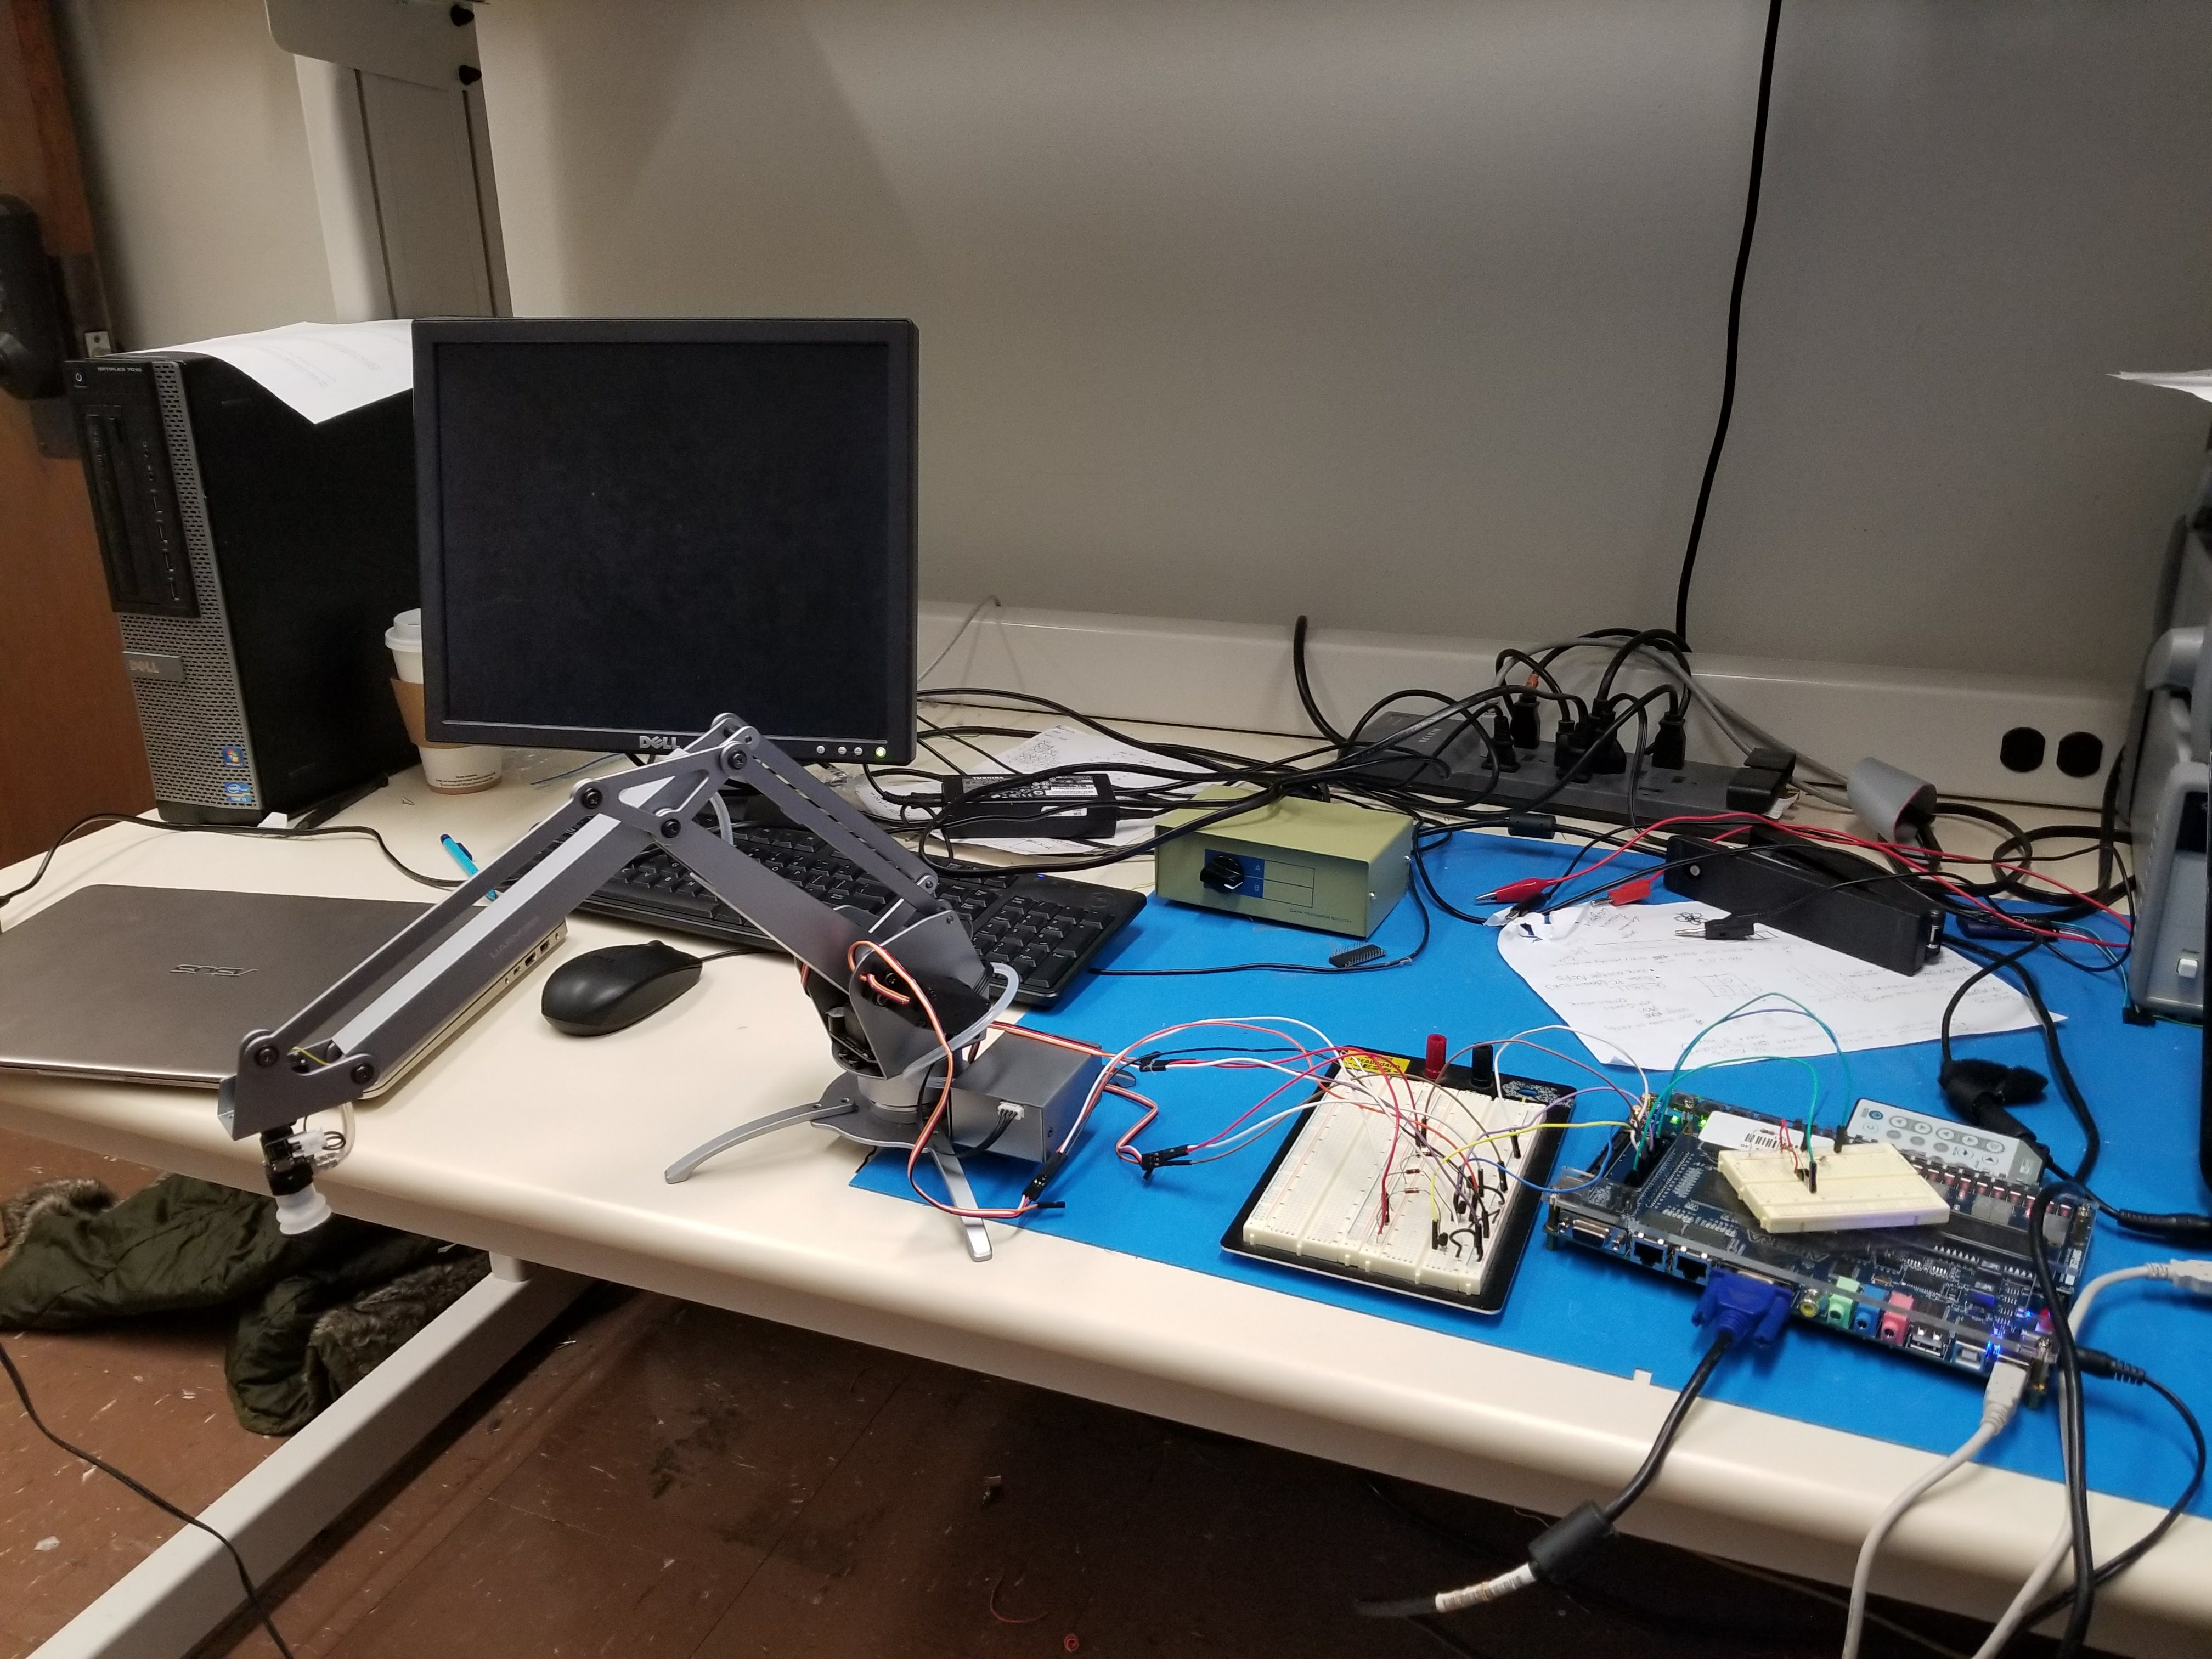
\includegraphics[scale=0.07]{setup.jpg}
        \caption{Full Setup of the Project}
        \label{fig:setup}
    \end{figure}
    
    \subsection{Input and Output Devices}

        \subsubsection{Robotic Arm}
        The robotic arm used was a uArm Metal, manufactured by uFactory. The arm can move in four planes of motion, controlled by one servomotor each, and also has a pump in order to pick up objects with suction. Only three of the planes of motion were used (X, Y, Z), and the pump was not enabled. These three directions of motions are described in Figure \ref{fig:armMotion}. The arm controller module includes a clock divider that reduces the clock frequency from 50 MHz to 50 Hz. A finite state machine modifies the pulse width linearly between 500 and 2500 microseconds, which corresponds to servomotor angles of 0-180 degrees. Figure \ref{fig:actualArm} shows a close-up picture of the arm in the setup.
        
        \begin{figure}[H]
            \begin{center}
                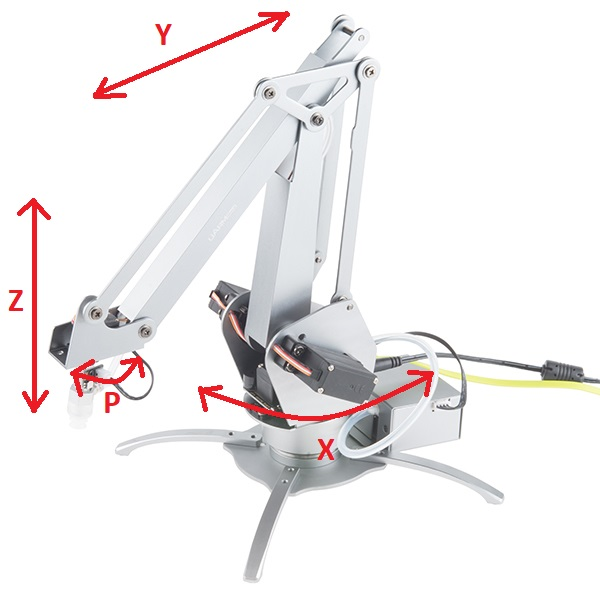
\includegraphics[scale=1]{armMotion.jpg}
                \caption{uArm Metal Planes of Motion}
                \label{fig:armMotion}
            \end{center}
        \end{figure}
        
        \begin{figure}[H]
            \centering
            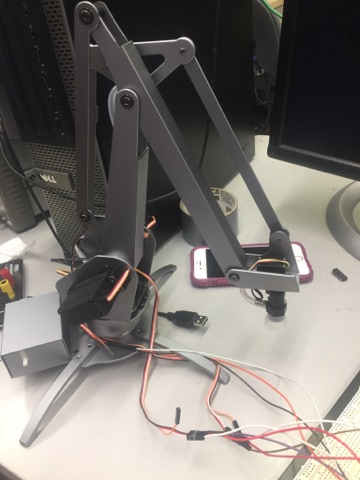
\includegraphics[scale=0.6]{arm.jpg}
            \caption{The Robotic Arm}
            \label{fig:actualArm}
        \end{figure}
       
       Since the arm operates on a 5 V pulse width modulation standard, and the GPIO pins on the FPGA could only supply 3.3 V signals, a common-emitter amplifier had to be constructed in order to amplify the 3.3 V signal to  5 V. Figure \ref{fig:amplifier} shows the circuit constructed. The constant 5 V and ground GPIO pins were used from the FPGA as power and ground for the circuit. Power, ground, and the output from the amplifier were connected to the servomotor. Figure \ref{fig:actualAmplifier} shows a picture of the amplifier circuits implemented.
       
       \begin{figure}[H]
            \begin{center}
                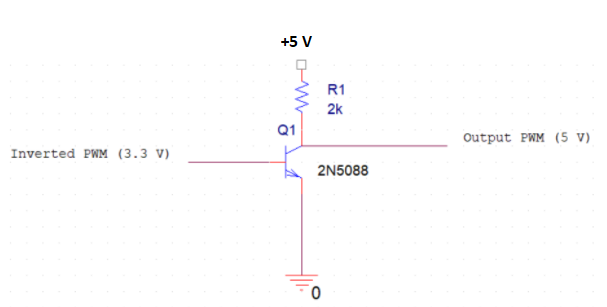
\includegraphics[scale=1]{amplifier.PNG}
                \caption{Common-Emitter Amplifier}
                \label{fig:amplifier}
            \end{center}
        \end{figure}
        
        \begin{figure}[H]
            \centering
            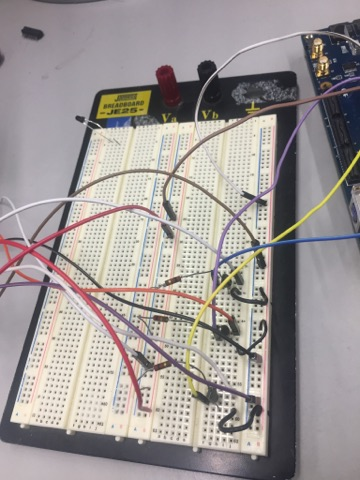
\includegraphics[scale=0.6]{amp.jpg}
            \caption{Implementation of the Common-Emitter Amplifiers}
            \label{fig:actualAmplifier}
        \end{figure}
        
        Since the amplifier has inverting gain, the PWM signal outputted from the processor had to be inverted, and the amplifier re-inverted the signal to give the proper pulse widths. Figure \ref{fig:pwm} shows an example of a valid PWM signal.
        
        \begin{figure}[H]
            \begin{center}
                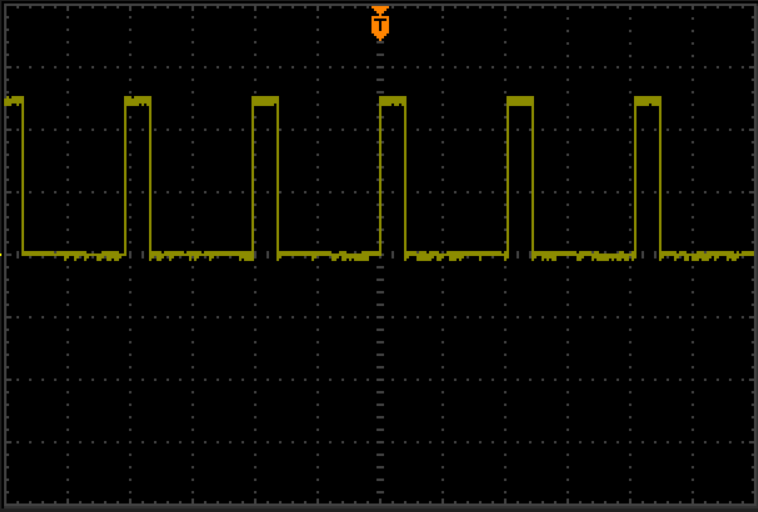
\includegraphics[scale=0.5]{pwm.PNG}
                \caption{Square Wave PWM Signal}
                \label{fig:pwm}
            \end{center}
        \end{figure}
        
        Finally, the angle of the servomotor is written to designated registers for the servomotor angles: {\tt \$r26} for {\tt servox}, {\tt \$r27} for {\tt servoy}, and {\tt \$r28} for {\tt servoz}.
        
    \subsubsection{Light Sensor}
    The light sensor circuit shown in Figure \ref{fig:lightSensor} was constructed with an NMOS common-source amplifier with a photoresistor as one of the gate resistances. The photoresistor increases its resistance to about 4 M$\Omega$ in darkness, and this reduces the gate voltage on the NMOS, turning it off. This removes the connection between the output and ground through the NMOS, and gives a high output voltage. In light, the photoresistor's resistance falls to around 100 $\Omega$, and this does the opposite, switching the NMOS on and pulling the output voltage low. Figure \ref{fig:actualLightSensor} shows a picture of the actual light sensor circuit built.
        
        \begin{figure}[H]
            \begin{center}
                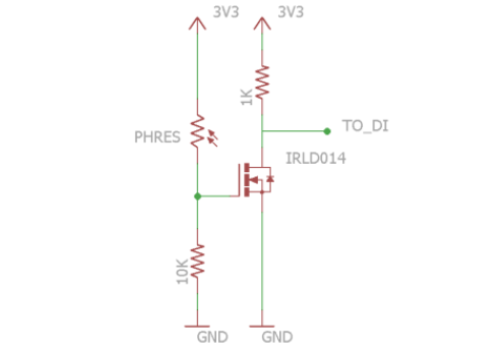
\includegraphics[scale=0.8]{lightSensor.PNG}
                \caption{Light Sensor Circuit}
                \label{fig:lightSensor}
            \end{center}
        \end{figure}
        
        \begin{figure}[H]
            \centering
            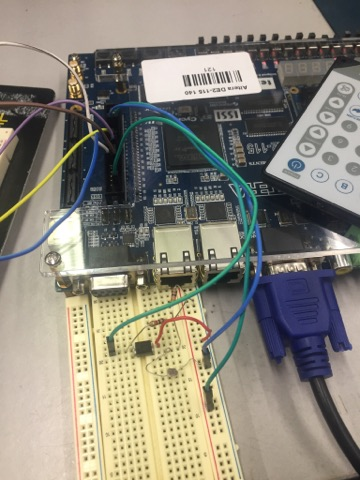
\includegraphics[scale=0.6]{lightpicsensor.jpg}
            \caption{Implementation of the Light Sensor}
            \label{fig:actualLightSensor}
        \end{figure}
        
    The constant 3.3 V and ground GPIO pins on the FPGA were used for the power and ground ports on the circuit. The output of the light sensor was passed into a GPIO pin, and was used as a reset signal for the processor. Triggering the light sensor reset requires almost complete darkness, so the sensor had to be almost completely covered.
    
    \subsubsection{Infrared Remote}
        The infrared remote packaged with the FPGA has a set of buttons with several buttons as shown in Figure \ref{fig:remote}. The numeric buttons were handled for the purposes of this project. 
    
        \begin{figure}[H]
            \begin{center}
                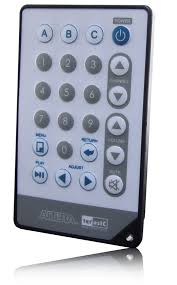
\includegraphics[scale=0.7]{remote.jpg}
                \caption{FPGA Infrared Remote}
                \label{fig:remote}
            \end{center}
        \end{figure}
        
        The infrared controller module was placed into the datapath like the robotic arm controller module. Data from the infrared remote came in a serial fashion, so it takes 34 cycles to process the data from the infrared remote: one for each bit that is transmitted. The data starts with a one bit lead code that indicates that data is being transmitted. Then, there is a custom code that is transmitted by a specific remote. Next, the key code bits are transmitted, and this is used to determine which key has been pressed. This is followed by the inverse of the key code for error-checking purposes. Finally, one bit is transmitted at the end to show that the information has finished transmitting. The key codes that correspond to each button press is shown in Figure \ref{fig:keycodes} below. The button type that was read out was then stored to a designated infrared register ({\tt \$r29}), and this was used later in the VGA Display (see below).
        
        \begin{figure}[H]
            \centering
            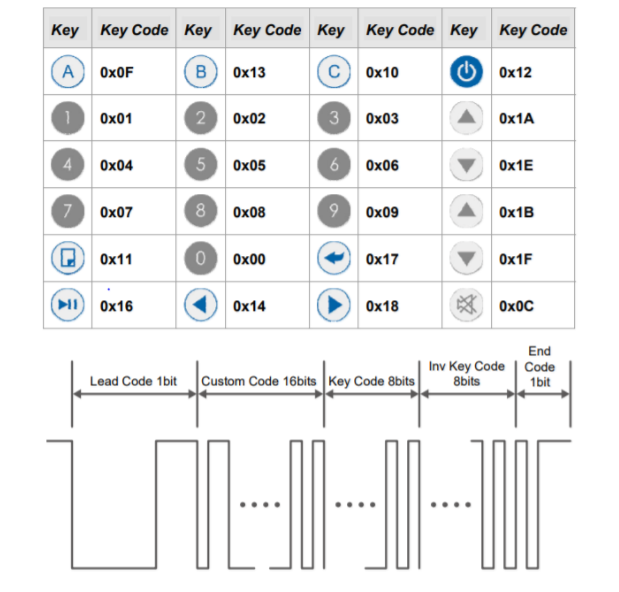
\includegraphics[scale=0.8]{keycodes.png}
            \caption{Infrared Remote Keycodes}
            \label{fig:keycodes}
        \end{figure}
    
    \subsubsection{VGA Display}
    The VGA display was able to change color based on the specific button that was pressed. The mappings of the numeric buttons on the remote to the hex value of the color is shown below in Table \ref{tbl:color}.
    
    \begin{table}[H]
        \centering
        \begin{tabular}{|c|c|} \hline
            \textbf{Number} & \textbf{Color} \\\hline
            0 & {\tt 0x7aff33} \\\hline
            1 & {\tt 0xff0000} \\\hline
            2 & {\tt 0xff8c33} \\\hline
            3 & {\tt 0xffff00} \\\hline
            4 & {\tt 0x00ff00} \\\hline
            5 & {\tt 0x0000ff} \\\hline
            6 & {\tt 0xff00ff} \\\hline
            7 & {\tt 0x9a00ff} \\\hline
            8 & {\tt 0x000000} \\\hline
            9 & {\tt 0x111111} \\\hline
        \end{tabular}
        \caption{Button to Color Mappings}
        \label{tbl:color}
    \end{table}
    
    The VGA controller was placed outside of the datapath, and read values of the button press from outputs from the processor. This module was designed based on the VGA skeleton code provided in Lab 7, but used constant color values instead of image .mif files to change the screen.
    
    \subsection{Changes to Processor}
    Changes were made to the processor in order to fix existing issues with control flow: jumps and branches were fixed in order to ensure proper operation. The {\tt bne} instruction was modified to {\tt beq} since it would have been more necessary for this project's purposes to check for equality between registers than inequality. For example, in the case of the infrared sensor, it made sense to check for equality with the type of button press. \\\hspace*{\fill}
    
    The modules for the robotic arm controller and infrared remote controller were embedded directly into the datapath, similar to how the mult/div module was included in the datapath. Instructions were added to move each of the servomotors ({\tt servox, servoy, servoz}) and read from the infrared sensor ({\tt ir}). Running any of the servo instructions would stall the pipeline for 1 million cycles in order to produce a 50 Hz pulse. Running the {\tt ir} instruction would stall for 34 cycles in order to read all of the data.
    
\section{Assembly Code}
    See the project repository for the assembly code used for the demo. The assembly code is very simplistic: in the first non-stall instruction, data is read from the infrared remote in order to determine which action the robotic arm must take. A branch instruction is called which is able to select between various robotic arm subroutines. Each subroutine moves the arm in a different way by calling on the servomotors to move to different angles. There are many no-ops inserted to ensure that the timing of the instructions occurs properly.

\section{Testing}
    Testing for control flow logic for the processor was conducted with vector waveforms, which can be found in the project repository. These showed all of the control signals of the processor at each stage, as well as the key outputs of execute, register file, etc. to help ensure that the proper outputs were being observed at each stage. The servomotor control module could also be debugged with vector waveforms; however, the number of cycles that the processor must stall to handle outputting a PWM signal was modified to a small number to ensure that the general timing was correct within the 1 microsecond limit of the waveform simulation. The amplifiers and light sensor circuit were debugged with using a triple output power supply and multimeter. Once the module was built and integrated with the processor, oscilloscopes could be used to ensure that the proper PWM signal was being outputted by the FPGA. Debugging the infrared module was difficult to do with vector waveforms since the output of a keypress is hard to emulate; because of this, most testing was done by blasting new iterations of the code to the FPGA and conducting multiple tests that way.
    
\section{Challenges}
    The main challenge with the robot arm was getting the arm to move at all. The arm came preassembled with an Arduino board, so measuring the PWM characteristics for the motor involved writing Arduino routines for the arm and using those to identify the necessary frequency and pulse widths. Once the PWM signal was established, it was then discovered that the FPGA could not output the proper amplitude for the pulse, which then led to the construction of the voltage amplifiers. Finally, it proved to be difficult to coordinate timing of the processor for the servo instructions since the million-cycle stalls occasionally led to some instructions getting "lost" during execution; this called for exstensive debugging of the processor.

    Similar timing issues were encountered with the infrared sensor. It was difficult to coordinate the 34 cycle stall and have the next few instructions line up after running an infrared instruction. It was also difficult to coordinate the timing of receiving all of the data from the infrared remote: with improper timing, the data was lost, and it was impossible to tell which button on the remote was pressed. All of these timing challenges were handled by carefully clocking every element at the proper frequency and at the proper edges so that the data was transmitted, received, and stored properly.

\section{References}
\begin{enumerate}
    \item Robot Arm Image: modified from https://cdn.sparkfun.com/assets/parts/1/1/0/9/1/13663-04.jpg\\\hspace*{\fill}
    \item Key Code table: \\ 
    ftp://ftp.altera.com/up/pub/Altera\_Material/13.0/Boards/DE2-115/DE2\_115\_User\_Manual.pdf\\
    \item PWM Image: \\
    http://michael-buschbeck.github.io/assets/2013-11-10-rigol-ds1052e-oscilloscope-pwm/scope-screen-\\basic.gif \\
    \item Controller Image: http://www.terasic.com.tw/attachment/archive/949/image/image\_2\_thumb.jpg
\end{enumerate}

\end{document}